

\documentclass[a4paper]{article}
\usepackage[letterpaper, margin=1in]{geometry} % page format
\usepackage{listings} % this package is for including code
\usepackage{graphicx} % this package is for including figures
\usepackage{amsmath}  % this package is for math and matrices
\usepackage{amsfonts} % this package is for math fonts
\usepackage{tikz} % for drawings
\usepackage{hyperref} % for urls
\usepackage{float}
\usepackage{amssymb}
\lstset{language=Python}
\begin{document}




\title{Homework 02 \LaTeX{} Sheet}

\author{Cameron Brenner}

\date{3/6/2019}

\maketitle

\section{Exercise 2.1}
In Exercise 2.1, we are given equation 2.1 which is
\begin{equation}
\epsilon (M, N, \delta) = \sqrt{\frac{1}{2N}ln\frac{2M}{\delta}}
\end{equation}
and we are given the value $\delta = 0.03$ 
\subsection{Part A.}
In part A. of Exercise 2.1, given equation 2.1, we are asked to find the number of examples, $N$, to make $\epsilon \leq 0.05$, and we are given $M = 1$. This can be done by solving for $N$.
\begin{align}
0.05  \geq & \sqrt{\frac{1}{2N}ln\frac{2}{0.03}} \\
ln\frac{2}{0.03} = 4.1997 \\
0.05 \geq & \sqrt{\frac{4.1997}{2N}}\\
0.05^2  \geq & \frac{4.1997}{2N}\\
.0025 \geq & \frac{4.1997}{2N}\\
\frac{.0025}{4.1997} \geq & \frac{1}{2N}\\
\frac{4.1997}{.0025} \geq & 2N\\
1679.88 \geq & 2N\\
839.94 \geq & N\\ 
\end{align}
So $N \leq 839.94$, meaning that is how many examples are needed to make  $\epsilon \leq 0.05$ when $M = 1$.
\subsection{Part B.}
In part A. of Exercise 2.1, we are asked to do the same thing as part A, but instead we are given $M = 100$.
\begin{align}
0.05  \geq & \sqrt{\frac{1}{2N}ln\frac{200}{0.03}} \\
ln\frac{200}{0.03} = 8.8049 \\
0.05 \geq & \sqrt{\frac{8.8049}{2N}}\\
0.05^2 \geq & \frac{8.8049}{2N}\\
.0025 \geq & \frac{8.8049}{2N}\\
\frac{.0025}{8.8049} \geq & \frac{1}{2N}\\
\frac{8.8049}{.0025} \geq & 2N\\
3521.96 \geq & 2N\\
1760.98 \geq & N\\ 
\end{align}
So $N \leq 1760.98$, meaning this is the upper bound of examples needed to get $\epsilon \leq 0.05$ when $M = 100$.
\subsection{Part C.}
In part C. of Exercise 2.1, we are asked to do the same thing as the above parts, but we are given $M = 10,000$.
\begin{align}
0.05  \geq & \sqrt{\frac{1}{2N}ln\frac{20000}{0.03}} \\
ln\frac{20000}{0.03} = 13.41 \\
0.05 \geq & \sqrt{\frac{13.41}{2N}}\\
0.05^2 \geq & \frac{13.41}{2N}\\
.0025 \geq & \frac{13.41}{2N}\\
\frac{.0025}{13.41} \geq & \frac{1}{2N}\\
\frac{13.41}{.0025} \geq & 2N\\
5364 \geq & 2N\\
2682 \geq & N\\ 
\end{align}
So $N \leq 2682$, meaning this is the upper bound of examples needed to get $\epsilon \leq 0.05$ when $M=10000$.
\section{Exercise 2.11}
In Exercise 2.11, we are asked, given $m_H(N) = N + 1$ so the $d_{vc} = 1$, to use the generalization bound to give a bound for $E_{out}$ with confidence of $90\%$. \\
The generalization bound is given as equation 2.12, which is 
\begin{equation}
    E_{out}(g) \leq E_{in}(g) + \sqrt{ \frac{8}{N}ln\frac{4m_H(N)}{\delta}}
\end{equation}
In the Exercise, we are told we have 100 training examples, so $N=100$, and because the confidence is $90\%$, $\delta = 0.1$.
\begin{align}
     E_{out}(g) \leq & E_{in}(g) + \sqrt{\frac{8}{100}ln\frac{4m_H(100)}{0.1}}\\
    E_{out}(g) \leq & E_{in}(g) + \sqrt{\frac{8}{100}ln\frac{4(101)}{0.1}}\\
    E_{out}(g) \leq & E_{in}(g) + \sqrt{\frac{8}{100}ln\frac{404}{0.1}}\\
    ln\frac{404}{.1} = 8.304\\
    E_{out}(g) \leq & E_{in}(g) + \sqrt{\frac{66.432}{100}}\\
    E_{out}(g) \leq & E_{in}(g) + \sqrt{.664}\\
    E_{out}(g) \leq & E_{in}(g) + 0.815\\
\end{align}
We are then asked to repeat finding the bound, but when there are 10,000 training examples, so now $N=10000$.
\begin{align}
     E_{out}(g) \leq & E_{in}(g) + \sqrt{\frac{8}{10000}ln\frac{4m_H(10000)}{0.1}}\\
    E_{out}(g) \leq & E_{in}(g) + \sqrt{\frac{8}{10000}ln\frac{4(10001)}{0.1}}\\
    E_{out}(g) \leq & E_{in}(g) + \sqrt{\frac{8}{10000}ln\frac{40004}{0.1}}\\
    ln\frac{40004}{.1} = 12.899\\
    E_{out}(g) \leq & E_{in}(g) + \sqrt{\frac{103.192}{10000}}\\
    E_{out}(g) \leq & E_{in}(g) + \sqrt{0.01}\\
    E_{out}(g) \leq & E_{in}(g) + 0.1\\
\end{align}
\section{Exercise 2.12}
In exercise 2.12 we have a hypothesis set $H$ with a $d_{vc}$ of 10. We are asked to find the sample size given $95\%$ confidence and a generalization error no more than 0.05. The equation we will use is equation 2.13, which is:
\begin{equation}
    N \geq \frac{8}{\epsilon^2}ln\frac{4((2N)^{d_{vc}} + 1)}{\delta}
\end{equation}
We then substitute $0.05$ for $\delta$ and $\epsilon$ and multiply out the 4 to simplify the equation a little. We also substitute the $d_{vc} = 10$.
\begin{equation}
    N \geq \frac{8}{0.05^2}ln\frac{4(2N)^{10} + 4}{0.05}
\end{equation}
We start by making an estimate for N, and then plugging the result into N again, and repeating until it converges to a sample size.
Assume $N=10,000$
\begin{align}
    N \geq & \frac{8}{0.05^2}ln\frac{4(2(10000)^{10} + 4}{0.05}\\
    N \geq & \frac{8}{0.0025}ln\frac{4(20000)^{10} + 4}{0.05}\\
    N \geq & \frac{8}{0.0025}ln\frac{4(a big number) + 4}{0.05}\\
    N \geq & \frac{8}{0.0025} * 100.421\\
    N \geq & 3200 * 100.421\\
    N \geq & 321347.2\\
\end{align}
So now we plug this number back into the equation.
\begin{align}
    N \geq & \frac{8}{0.05^2}ln\frac{4(2(321347.2)^{10} + 4}{0.05}\\
    N \geq & \frac{8}{0.0025}ln\frac{4(642694.4)^{10} + 4}{0.05}\\
    N \geq & \frac{8}{0.0025}ln\frac{4(1.2023895e+58) + 4}{0.05}\\
    N \geq & \frac{8}{0.0025} * 138.116\\
    N \geq & 3200 * 138.116\\
    N \geq & 441972.073\\
\end{align}
We are getting closer so now we plug this number in for $N$.
\begin{align}
    N \geq & \frac{8}{0.05^2}ln\frac{4(2(441972.073)^{10} + 4}{0.05}\\
    N \geq & \frac{8}{0.0025}ln\frac{4(883944.146)^{10} + 4}{0.05}\\
    N \geq & \frac{8}{0.0025}ln\frac{4(2.9123813e+59) + 4}{0.05}\\
    N \geq & \frac{8}{0.0025} * 141.304\\
    N \geq & 3200 * 141.304\\
    N \geq & 452172.8\\
\end{align}
The difference is getting noticeably smaller so we will try one more time before giving an estimate
\begin{align}
    N \geq & \frac{8}{0.05^2}ln\frac{4(2(452172.8)^{10} + 4}{0.05}\\
    N \geq & \frac{8}{0.0025}ln\frac{4(904345.6)^{10} + 4}{0.05}\\
    N \geq & \frac{8}{0.0025}ln\frac{4(3.6588474e+59) + 4}{0.05}\\
    N \geq & \frac{8}{0.0025} * 141.531\\
    N \geq & 3200 * 141.532\\
    N \geq & 452902.4\\
\end{align}
This answer is very similar to the last one, so we can now give an estimate for N, which is $N \approx 450,000$, meaning with a confidence of $95\%$ and a generalization error of at most 0.05, we need a sample size around 450,000. 
\section{Exercise 3.1}
In Exercise 3.1 we are given two semi-circles from Dr. Rivas's code and told to set $rad = 10, thk = 5, sep = 5$ for the exercise.
\subsection{Part A.}
In Part A, we are asked to run the PLA on the semi circles and plot our results. 
\begin{figure}[H]
    \begin{center}
        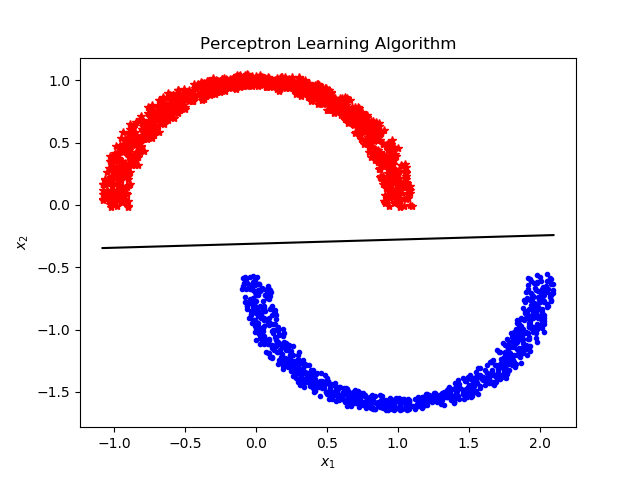
\includegraphics[width=0.75\textwidth]{hw02pla.png}
    \end{center}
    \label{fig:partapla}
\end{figure}
Here are the misclassified points for the PLA.
\begin{figure}[H]
    \begin{center}
        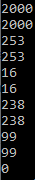
\includegraphics[width=0.05\textwidth]{hw02pladata.PNG}
    \end{center}
    \label{fig:partapladata}
\end{figure}
\subsection{Part B.}
In Part B, we are asked to do the same thing but with linear regression, using the code given from the lab.
\begin{figure}[H]
    \begin{center}
        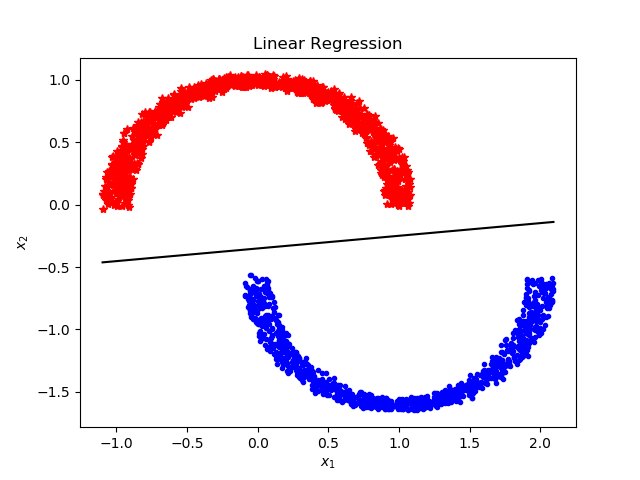
\includegraphics[width=0.75\textwidth]{hw02linreg.png}
    \end{center}
    \label{fig:partblinreg}
\end{figure}
Here are the data points for the linear regression.
\begin{figure}[H]
    \begin{center}
        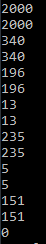
\includegraphics[width=0.05\textwidth]{hw02linregdata.PNG}
    \end{center}
    \label{fig:partblinregdata}
\end{figure}
The difference in the PLA and Lin Reg is interesting. In the LinReg model, the closer inside parts of the semi circles are closer to the solution line that linear regression gives, and the ends on the farther end are farther apart from the solution, while on the PLA, all ends of the semicircles seem to be equally far apart from the PLA. Although the linear regression model seemed to have run a little longer, it seems the more accurate of the two. 

\end{document}